\documentclass[conference]{IEEEtran}
\IEEEoverridecommandlockouts
% The preceding line is only needed to identify funding in the first footnote. If that is unneeded, please comment it out.
\usepackage{cite}
\usepackage{amsmath,amssymb,amsfonts}
\usepackage{algorithmic}
\usepackage{graphicx}
\usepackage{textcomp}
\usepackage{xcolor}
\usepackage{balance}

\usepackage[nohyperlinks, printonlyused, nolist]{acronym}

\usepackage[utf8]{inputenc}
\usepackage[T1]{fontenc} % Trennen von Wörtern mit Umlauten
\usepackage{ngerman} % Damit z.B. "Literatur" statt "References" da steht


\def\BibTeX{{\rm B\kern-.05em{\sc i\kern-.025em b}\kern-.08em
    T\kern-.1667em\lower.7ex\hbox{E}\kern-.125emX}}
\begin{document}

\begin{acronym}
    \acro{apt}[APT]{Advanced Persistent Threat}
\end{acronym}


\title{Methoden und Techniken von \aclp*{apt} am Beispiel des Solarwinds Compromise
}

\author{\IEEEauthorblockN{Laurenz Stinner}
    \IEEEauthorblockA{\textit{Fakultät für Informatik} \\
        \textit{Technische Hochschule Rosenheim}\\
        Rosenheim, Germany \\
        laurenz.p.stinner@stud.th-rosenheim.de}
}

\maketitle

\begin{abstract}

    Am des Solarwinds Compromise der \acs*{apt} 29 wird gezeigt, welche Methoden und Techniken durch \acsp*{apt} angewandt werden.
    ?? Deshalb ist es für Organisationen und Firmen unerlässlich sich gegen böswillige Akteure zu schützen.

    Paper soll anhand des Solarwinds Compromise der \ac{apt} 29 zeigen, wie diese Vorgehen, welche Techniken verwendet werden und welche Ziele APTs verfolgen.
    ?? Im Schlussteil werden die wichtigsten Maßnahmen aufgezeigt oder eine raffinierte Maßnahme im Detail erklärt
\end{abstract}

\begin{IEEEkeywords}
    \ac{apt}, Solarwinds, Cybersecurity, Machine Learning, Artificial Intelligence
\end{IEEEkeywords}

\section{Einführung}
Als \acp{apt} werden Gruppierungen oder Personen bezeichnet, die über ein hohes Maß an Fachwissen und erhebliche Ressourcen verfügen, die es Ermöglichen mehrere Angriffsvektoren zu nutzen.
Zusätzlich verfolgen \acp{apt} ihre Ziele wiederholt über einen längeren Zeitraum, passen sich den Bemühungen der Verteitiger an und sind entschlossen die Ziele zu erreichen.
Zu diesen Zielen gehören u.~a. das Exfiltrieren von Informationen, kritische Aspekte einer Organisation zu stören und sich im System des Ziels zu verbreiten und festzusetzen \cite[S.~B-1]{NIST2011}.
Die geschätzten jährlichen Kosten von Cyberkriminalität sollen laut Statista im Jahr 2023 auf 8,15 Billionen US-Dollar belaufen und bis 2028 um 69,94\% auf 13.82 Billionen US-Dollar steigen \cite{Statista2023}.


\subsection{Organisierte Kriminalität, Hacker und \aclp*{apt}}
Abgrenzung von \ac{apt} zu anderen Formen der Cyberkriminalität ist in Abb.~\ref{fig.destinction} dargestellt.
\begin{figure}[htbp]
    \centerline{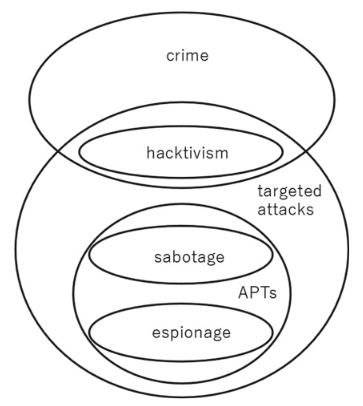
\includegraphics[scale=0.8]{figures/Destinction between targeted attacks, activity by APTs, and cyber-espionage.png}}
    \caption{Unterscheidung zwischen gezielten Angriffen, Aktivitätes von \acp{apt} und Cyberspionage \protect\cite[S.~6]{Steffens2020}}
    \label{fig.destinction}
\end{figure}
\subsection{Solarwinds Compromise}

\section{Vorgehensweise von \aclp{apt}}
Die Techniken der \acp{apt} werden immer komplexer und vielfältiger und bestehen aus vielschichtigen und zeitaufwändigen Prozessen \cite[S.~7f]{Steffens2020}.
Um sie besser zu verstehen, werden die verschiedenen Teile eines Anriffs in eine \textit{killchain} sortiert \cite[S.~8]{Steffens2020}, siehe Abb.~\ref{fig.killchain}.
\begin{figure}[htbp]
    \centerline{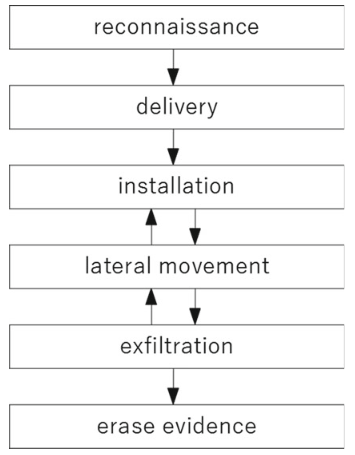
\includegraphics[scale=0.8]{figures/killchain.png}}
    \caption{Killchain: Idealisiertes Modell der Stufen eines \ac{apt}-Angriffs \cite[S.~8]{Steffens2020}}
    \label{fig.killchain}
\end{figure}
Es gibt weitere Killchain-Modelle, u.~a. von Lockheed Martin \cite{LockheedMartin}, welche einfachheitshalber nicht weiter in betracht genommen wurden.
\subsection{Aufkärung}
Das Ziel des ersten Schritts ist es nicht nur Information über das Ziel zu finden, sondern auch das Ziel festzulegen.
Wie und warum Ziele ausgewählt werden lässt sich schwer bis nicht feststellen.
Meist wird angenommen, dass \acp{apt} einen Auftrag durch Kunden bekommen, beispielsweise durch Geheimdienste, und danach ihre Ziele suchen.
Nachdem das Ziel feststeht beginnt die weitere Aufklärung.
Vgl. zu diesem Abschnitt Steffens \cite[S.~10-13]{Steffens2020}.
In der Regel werden öffentlich zugängliche Informationen über ein Ziel gesammelt, um dessen Arbeitsweise besser zu verstehen und potenzielle Angriffsvektoren zu identifizieren \cite{Cole2013}.
MITRE \cite{MITREReconnaissance} listet zehn Techniken auf, mit deren Hilfe Informationen über das Ziel gefunden werden können:
\begin{itemize}
    \item \textbf{Active Scanning} - Direkte Interaktion mit der Infrastruktur des Ziels (IP-Adressblöcke finden, Schwachstellenscanns, Wortlistsuche)
    \item \textbf{Gather Victim Host Informatiomn} - Harware- und Softwareinformation über das Zielsystem finden (Betriebssystem, Konfigurationen, Firmware, usw.)
    \item \textbf{Gather Victim Identity Information} - Informationen über Mitarbeiter (Daten von Personen, E-Mail Adressen, Zugangsdaten)
    \item \textbf{Gather Victim Network Information} - Grundlegende Informationen über das Netzwerk (IP-Adressen, DNS- \& Domain-Informationen, Netzwerktopologie, usw.)
    \item \textbf{Gather Victim Org Information} - Informationen über das Unternehmen sammeln, die für weiter Schritte genutzt werden können (Geschäftsbeziehungen, Personalstruktur und -hierarchie, usw.)
    \item \textbf{Phishing for Information} - Erlangen von vertraulichen Informationen mithilfe von u.~a. Social-Engineering Taktiken (Telefonate, E-Mails, usw.)
    \item \textbf{Search Closed Sources} - Informationen über das Ziel kaufen (Dark-Web Schwarzmärkte, usw.)
    \item \textbf{Search Open Technical Databases} - Technische Informationen über das Ziel in frei verfügbaren Online-Datenbanken finden (WHOIS, DNS, CDNs, usw.)
    \item \textbf{Search Open Websites/Domains} - Informationen über Suchmaschienen, Social-Media oder Coderepositorien finden.
    \item \textbf{Search Victim-Owned Websites} - Durchsuchen von Webseiten nach Informationen, die dem Ziel gehören (E-Mail Adressen, Mitarbeitername, usw.)
\end{itemize}
Viele der Techniken werden kombiniert, um am Ende das eigentliche Ziel zu erreichen.
Beispielsweise werden auf der Webseite des Ziels wichtigen Mitarbeitern gesucht, weitere Informationen über Social-Media gewonnen, um anschließend vertrauliche Informationen über das Ziel mittels Social-Engineering Taktiken zu gewinnen.

?? Solarwinds Compromise

\subsection{Auslieferung}
Die Auslieferung ist sehr verbunden mit der Aufklärung.
Häufig wird für eine gewählte Auslieferungsstrategie entsprechende Aufklärung durchgeführt.
??
Vgl. zu diesem Abschnitt Steffens \cite[S.~10-13]{Steffens2020}.
MITRE \cite{MITREInitialAccess} bezeichnet diesen Schritt als initialen Zugriff und unterscheidet zwischen zehn Techniken:
\begin{itemize}
    \item \textbf{Content Injection} - Nutzen von bereits kompromittierten Datenübertragungskanälen.
    \item \textbf{Drive-by Compromise} - Ziel wird aktiv zu bösartigen Nutzdaten auf einer kompromittierten Webseite gelockt, z.~B. Abgreifen von Anwendungszugriffstoken.
    \item \textbf{Exploit Public-Facing Application} - Ausnutzen einer Schwachstelle eines Systems.
    \item \textbf{External Remote Services} - Nutzen von unzureichend abgesicherten Remote-Diensten, wie VPNs.
    \item \textbf{Harware Additions} - Einbringen neuer Hardwaer in ein System oder Netzwerk, z.~B. Wechseldatenträger.
    \item \textbf{Phishing} - Versenden von Phishing-Nachrichten, um einen Zugang zum System des Ziels zu erhalten.
    \item \textbf{Replication Through Removable Media} - Eindringen in abgetrennte Netzwerke, z.~B. mittels Wechselmedien in Kombination mit Autorun-Funktionen
    \item \textbf{Supply Chain Compromise} - Einschleusen von bösartigem Code durch Auslieferungsmechanismen von Anwendungen.
    \item \textbf{Trusted Relationship} - Ausnutzen von vertrauenswürdigen Dritten, um Zugang zu einem Netzwerk zu erhalten.
    \item \textbf{Valid Accounts} - Nutzen von Anmeldeinformationen bestehender Konten (VPNs, Outlook, Remote-Desktop, ...)
\end{itemize}

?? Solarwinds compromis supply chain compromise

\subsection{Installation}
??
MITRE \cite{MITREEnterpriseTactics} unterscheidet in diesem Punkt zwischen Taktiken für die Ausführung von schadhaftem Code, \textit{Execution}, und Taktiken, um den Zugriff auf längere Zeit zu sichern \cite{MITREEnterpriseTactics}.
Zu den Taktiken für die Ausführung von schadhaftem Code listet MITRE \cite{MITREExecution} folgende auf:
\begin{itemize}
    \item \textbf{Cloud Administration Command} - Missbrauchen von Cloud-Verwaltungsdiensten, wie AWS Systems Manager und Azure Runcommand.
    \item \textbf{Command and Scripting Interpreter} - Befehls- und Skriptinterpreter, wie Unix-Shell und PowerShell, werden zum ausführen von schadhafem Code verwendet.
    \item \textbf{Container Administration Command} - Über Containerverwaltungsdienste kann schadhafter Code innerhalb eines Containers ausgeführt werden.
    \item \textbf{Deploy Container} - Einsetzen von schadhaften Containern, um beispielsweise Prozesse auszuführen die Malware ausführen oder herunterladen.
    \item \textbf{Exploitation for Client Execution} - Ausnutzern von Software-Schwachstellen in Client-Anwendungen, um Code auszuführen.
    \item \textbf{Inter-Process Communication} - Manipulieren von prozessübergreifender Kommunikation, um Befehle oder Code auszuführen.
    \item \textbf{Native API} - Verwenden von nativen Betriebssystemschnittstellen.
    \item \textbf{Scheduled Task/Job} - Ermöglicht bösartigen Code erstmalig oder wiederholt auszuführen, indem Fuktionen zur Aufgabenplanung missbraucht werden.
    \item \textbf{Serverless Execution} - Missbrauchen von Serverless Computing, Integrations- und Automatisierungsdiensten, um Code in Cloudumgebungen auszuführen.
    \item \textbf{Shared Modules} - Schadhafter Code kann über gemeinsame Module (z.~B. DLLs) ausgeführt werden.
    \item \textbf{Software Deployment Tools} - Bei Zugang zu installierten drittanbieter Softwares für Systemadministration, -monitoring und Softwarebereitstellung kann beliebe Malware in großen Teilen des Netzwerks installiert werden. Dadurch wird auch die Verbreitung im Netzwerk erzielt.
    \item \textbf{System Services} - Verwenden von Systemdiensten oder Daemons zur Ausführung von Code. Kann bereits zum erreichen von Persistenz verwendet werden.
    \item \textbf{User Execution} - Bösartiger Code wird hierbei durch einen Benutzer ausgeführt, der durch Social Engineering dazu gebracht wurde.
    \item \textbf{Windows Management Instrumentation} - Ausnutzen der Windows Management Insturmentation, um Befehle auszuführen.
\end{itemize}
Die größte Teil der genannten Taktiken ermöglichen es, schadhaften Code einmalig auszuführen, jedoch werden diese Prozesse nach neustart eines Systems beendet.
Um den Zugang über Neustarts hinweg zu sichern, werden Taktiken zu persistierung eingesetz \cite{MITREPersistence}.
Dazu gehören nach MITRE \cite{MITREPersistence} folgende Taktiken:
\begin{itemize}
    \item \textbf{Account Manipulation} - Aktionen um den Zugriff auf ein Konto aufrechtzuerhalten. z.~B. durch Ändern von Anmeldedaten.
    \item \textbf{BITS Jobs} - Windows Brackground Intelligent Transfer Services (BITS) können genutzt werden um Malware als Hintergrundaufgabe dauerhaft auszuführen.
    \item \textbf{Boot or Logon Autostart Execution} - Systemeinstellungen konfigurieren, damit ein Programm bei Systemstart oder Anmeldung automatisch ausgeführt wird.
    \item \textbf{Boot or Logon Initialization Scripts} - Verwendung von Skripten die automatisch beim Booten oder bei der Anmeldung auseführt werden.
    \item \textbf{Browser Extensions} - Missbrauchen von Browser-Erweiterungen, um sich dauerhaften Zugang zu verschaffen.
    \item \textbf{Compromise Client Software Binary} - Schadhaften Code in Client-Software-Binärdateien einschleusen.
    \item \textbf{Create Account} - Eigenes Konto für den Systemzugang erstellen.
    \item \textbf{Create or Modify System Process} - Erstellen oder Ändern von Prozessen auf Systemebene (z.~B. Windows-Dienste). Diese werden beim Start des Betriebssystems hochgefahren.
    \item \textbf{Event Triggered Execution} - Mit Hilfe von Systemmechanismen können bei bestimmten Ereignissen Prozesse ausgeführt werden. Besonders in Cloud-Umgebungen, werden Cloud-Ereignisse überwacht und bei entsprechende Ereignissen Funktionen oder Dienste ausgeführt.
    \item \textbf{External Remote Services} - Über Remote-Dienste kann der Zugriff auf ein Netzwerk persistiert werden (z.~B. VPNs).
    \item \textbf{Hijack Execution Flow} - Missbrauch der Art und Weise, wie Betriebssystem Programme ausführen (Ausführungsfluss). Durch umgeleitete Ausführungen kann schadhafter Code immer wieder geladen werden.
    \item \textbf{Implant Internal Image} - Einsetzen von schadhaftem Code in Cloud- oder Container-Images.
    \item \textbf{Modify Authentication Process} - Modifizieren von Authentifizierungsmechanismen- und -prozessen, um auf Benutzeranmeldeinformationen zuzugreifen.
    \item \textbf{Office Application Startup} - Verwendung von Office-Vorlagenmakros oder Add-Ins, um schadhaften Code in Office-basierten Anwendungen zu persistieren.
    \item \textbf{Power Settings} - Beeinträchtigen der Systemfunktionen in den Ruhezustand zu gehen, neu zu starten oder herunterzufahren, um zu verhindern, dass schadhafter Code gestoppt wird.
    \item \textbf{Pre-OS Boot} - Nutzen von Pre-OS-Boot-Mechanismen, um während des Bootvorgangs schadhafte Firmware und verschiedene bösartige Startdienste vor dem Betriebssystem zu laden.
    \item \textbf{Scheduled Task/Job} - Erstellen oder Modifizieren von geplanten Aufgaben, um schadhaften Code wiederholt auszuführen.
    \item \textbf{Server Software Component} - Ausnutzen von legitimen, erweiterbaren Entwicklungsfunktionen von Servern, die ermöglichen Software oder Skripte zu schreiben und zu installieren.
    \item \textbf{Traffic Signaling} - Verbergen von offenen Ports oder anderen bösartigen Funktionen. Ein magischer Wert oder eine Sequenz muss verwendet werden, um eine Reaktion auf dem System auszulösen, z.~B. das Öffnen eines Ports oder die Ausführung einer bösartigen Aufgabe.
    \item \textbf{Valid Accounts} - Durch erbeutete Anmeldeinformationen bestehender Konten, können diese Wiederholt missbraucht werden, um den Zugriff aufrechtzuerhalten.
\end{itemize}

\subsection{Verbreitung}
MITRE \cite{MITRELateralMovement} unterscheidet dabei zwischen folgenden Taktiken:
\begin{itemize}
    \item \textbf{Exploitation of Remote Services} - Ausnutzen eines Remote-Dienstes innerhalb eines Netzwerkes, um sich unerlaubten Zugang zu weiteren internen Systemen zu verschaffen. Dabei werden Software-Schwachstellen in Programmen und Betriebssystemen ausgenutzt.
    \item \textbf{Internal Spearphishing} - Angreifer können sich mittels internem Spearphishing Zugang zu zusätzlichen Information verschaffen. Es handelt sich dabei um ein mehrstufiges Verfahren, bei dem z.~B. ein E-Mail-Konto eines Benutzers in Besitz genommen wird.
    \item \textbf{Lateral Tool Transfer} - Übertragen von Tools oder anderen Dateien zwischen Systemen in einer kompromittierten Umgebung.
    \item \textbf{Remove Service Session Hijacking} - Kontrolle über bereits bestehende Sitzungen in Remote-Diensten übernehmen.
    \item \textbf{Remote Services} - Verwenden von gültigen Kontent, um sich bei einem Dienst anzumelden, der Remote-Verbindungen akzteptiert, z.~B. SSH.
    \item \textbf{Replication Through Removable Media} - Wechselmedien können verwendet werden, um sich auch in getretten Netzwerken zu verbreiten. Dabei wird Malware auf das Wechselmedium gespielt und mittels Autorun-Funktion auf dem getrennten System ausgeführt.
    \item \textbf{Software Deployment Tools} - Zugang zu Softwarebereitstellungssystemen von Drittanbietern zu verschaffen, um diese zur Verbreitung zu nutzen.
    \item \textbf{Taint Shared Content} - Schadprogramme auf gemeinsam genutzten Speicherorten (Netlaufwerke, Code-Repositorien) in vertrauenswürdigen Dateien ablegen. Sobald ein Nutzer den freigegebenen Inhalt öffnet, kann so der Schadcode verbreitet werden.
    \item \textbf{Use Alternate Authentication Material} - Verwenden von alternativem Authentifizierungsmaterial (Kennwort-Hashes, Kerberos-Tickets, Token, usw.), um sich weiter im System zu verbreiten.
\end{itemize}

\subsection{Exfiltration}
?? \cite{MITREExfiltration}
\begin{itemize}
    \item \textbf{Automated Exfiltration} - Automatisches exfiltrieren von z.~B. sensiblen Dokumenten. Dafür wird diese Technik meist mit anderen Exfiltrationstechniken kombiniert \cite{MITREAutomatedExfiltration}.
    \item \textbf{Data Transfer Size Limit} - Exfiltrieren von Daten in kleineren Paketen, um z.~B. zu vermeiden, dass Schwellenwerte für die Datenübertragung im Netzwerk nicht überschritten werden.
    \item \textbf{Exfiltration Over Alternative Protocol} - Daten über andere Protokolle, als das der bestehenden Verbindung, exfiltrieren.
    \item \textbf{Exfiltration Over C2 Channel} - Daten über das Protokol der bestehenden Verbindung exfiltrieren.
    \item \textbf{Exfiltration Over Other Network Medium} - Nutzen von anderen Netwerkmedien, wie WiFi-Verbindungen, mobile Datenverbindungen oder Bluetooth, um Daten zu exfiltrieren.
    \item \textbf{Exfiltration Over Physical Medium} - Stehlen von Daten mittels physischer Medien, z.~B. USB-Laufwerke oder Mobiltelefone.
    \item \textbf{Exfiltration Over Web Services} - Verwenden von Webdiensten zur Exfiltration, z.~B. über Fileshare-Dienste.
    \item \textbf{Scheduled Transfer} - Planen von Datenexfiltrationen, damit nur zu bestimmten Tageszeiten oder in bestimmten Zeitabständen. Diese Taktik wird u.~U. genutzt, um den Datenverkehr mit normalen Aktivitäten zu vermischen. Andere Taktiken werden meist mit dieser verbunden \cite{MITREScheduledTransfer}.
    \item \textbf{Transfer Data to Cloud Account} - Übertragen von Daten, einschließlich Backups von Cloud-Umgebungen, auf ein anderes Cloud-Konto, um Exfiltrationserkennung zu umgehen.
\end{itemize}
\subsection{Beweise löschen}

\section{Vorgehensweise im Solarwinds Compromise}

\section{Verteidigung gegen \aclp{apt}}
\subsection{Threat Hunting}
\subsection{Visual Analytics with the MASFAD framework}
\section{Fazit ??}

\section*{Acknowledgment}

\section*{References}

\balance
\bibliographystyle{IEEEtran}
\bibliography{IEEEexample}



\vspace{12pt}
\color{red}
IEEE conference templates contain guidance text for composing and formatting conference papers. Please ensure that all template text is removed from your conference paper prior to submission to the conference. Failure to remove the template text from your paper may result in your paper not being published.

\end{document}
